\section{VPNs}

A VPN creates a secure channel between two networks over an untrusted network (the Internet). VPNs and end-to-end security (TLS) complement each other. Many different VPN protocols and applications exist.
(IPsec, Strongswan, OpenVPN, WireGuard, ...)
\begin{itemize}
    \item \textbf{Set-up phae:} Tunnel endpoints authenticate each other and set up keys (similar to TLS handshake
    \item \textbf{Tunneling phase:} Packets are encapsulated at the first endpoint and decapsulated at the second. The original packet is (often) encrypted and authenticated with a MAC.
\end{itemize}

\paragraph{Typical properties of VPN tunnels:}
\begin{itemize}
	\item Similar security properties as the TLS record protocol:
	\begin{itemize}
		\item Authentication of the source, integrity (MACs)
		\item Confidentiality (symmetric encryption)
		\item Replay suppression (sequence numbers)
	\end{itemize}
	\item Some tunneling protocols do not provide encryption or authentication
\end{itemize}

\paragraph{Typical VPN setups:}
\begin{itemize}
	\item site-to-site: secure connection between two physically separated networks.  
	\item host-to-site: secure connection of a remote host to company/university network. Private IP addresses can be accessed without port forwarding. Services do not need to be exposed to the internet. All traffic between Host and private network is secure.
	\item VPN as a “secure” proxy (avoid tracking, spoof location, circumvent censorship)
\end{itemize}

\paragraph{VPN does not provide anonymity:} 
\begin{itemize}
    \item Local network and ISP do not see which websites you access.
    \item VPN server can monitor and record all traffic.
\end{itemize}

\paragraph{Why do we need VPNs when we have TLS?}
\vspace{-\topsep}
\begin{itemize}
	\item If we only want to operate on layer 3 (e.g. company printer network) and still be secure
	\item When only using TLS: we still leak metadata
	\item HTTPS doesn't hide layer 3 information (srcIP, dstIP)
	\item VPNs protect all traffic ('blanket' security): DNS requests, accessing webservers without TLS
	\item VPNs can give access to services in private networks or behind firewalls
	\item VPNs allow to spoof your location
\end{itemize}

\paragraph{Why do we need TLS when we have VPNs?}
\begin{itemize}
	\item With VPNs, data is only secure inside the tunnel. But the data needs to somehow get to and from the tunnel. VPNs provide no security outside the tunnel
	\item VPN server can see all unencrypted traffic. TLS is still necessary.
	\item With a VPN it is not possible to authenticate a webserver, only the tunnel endpoint.
	\item VPNs need initial credential setup, TLS can be setup without knowing each other
\end{itemize}

\paragraph{There are many different VPN protocols but only one TLS. Why?}
Because TLS is universal, everybody should be able to access webservers securely through TLS.  We thus need a globally universal standard. VPNs are setup by companies, universities, private person etc. and it only affects their clients, employees etc.. For VPNs, we can thus use whatever we want.

\begin{minipage}{\linewidth}
    \centering      
    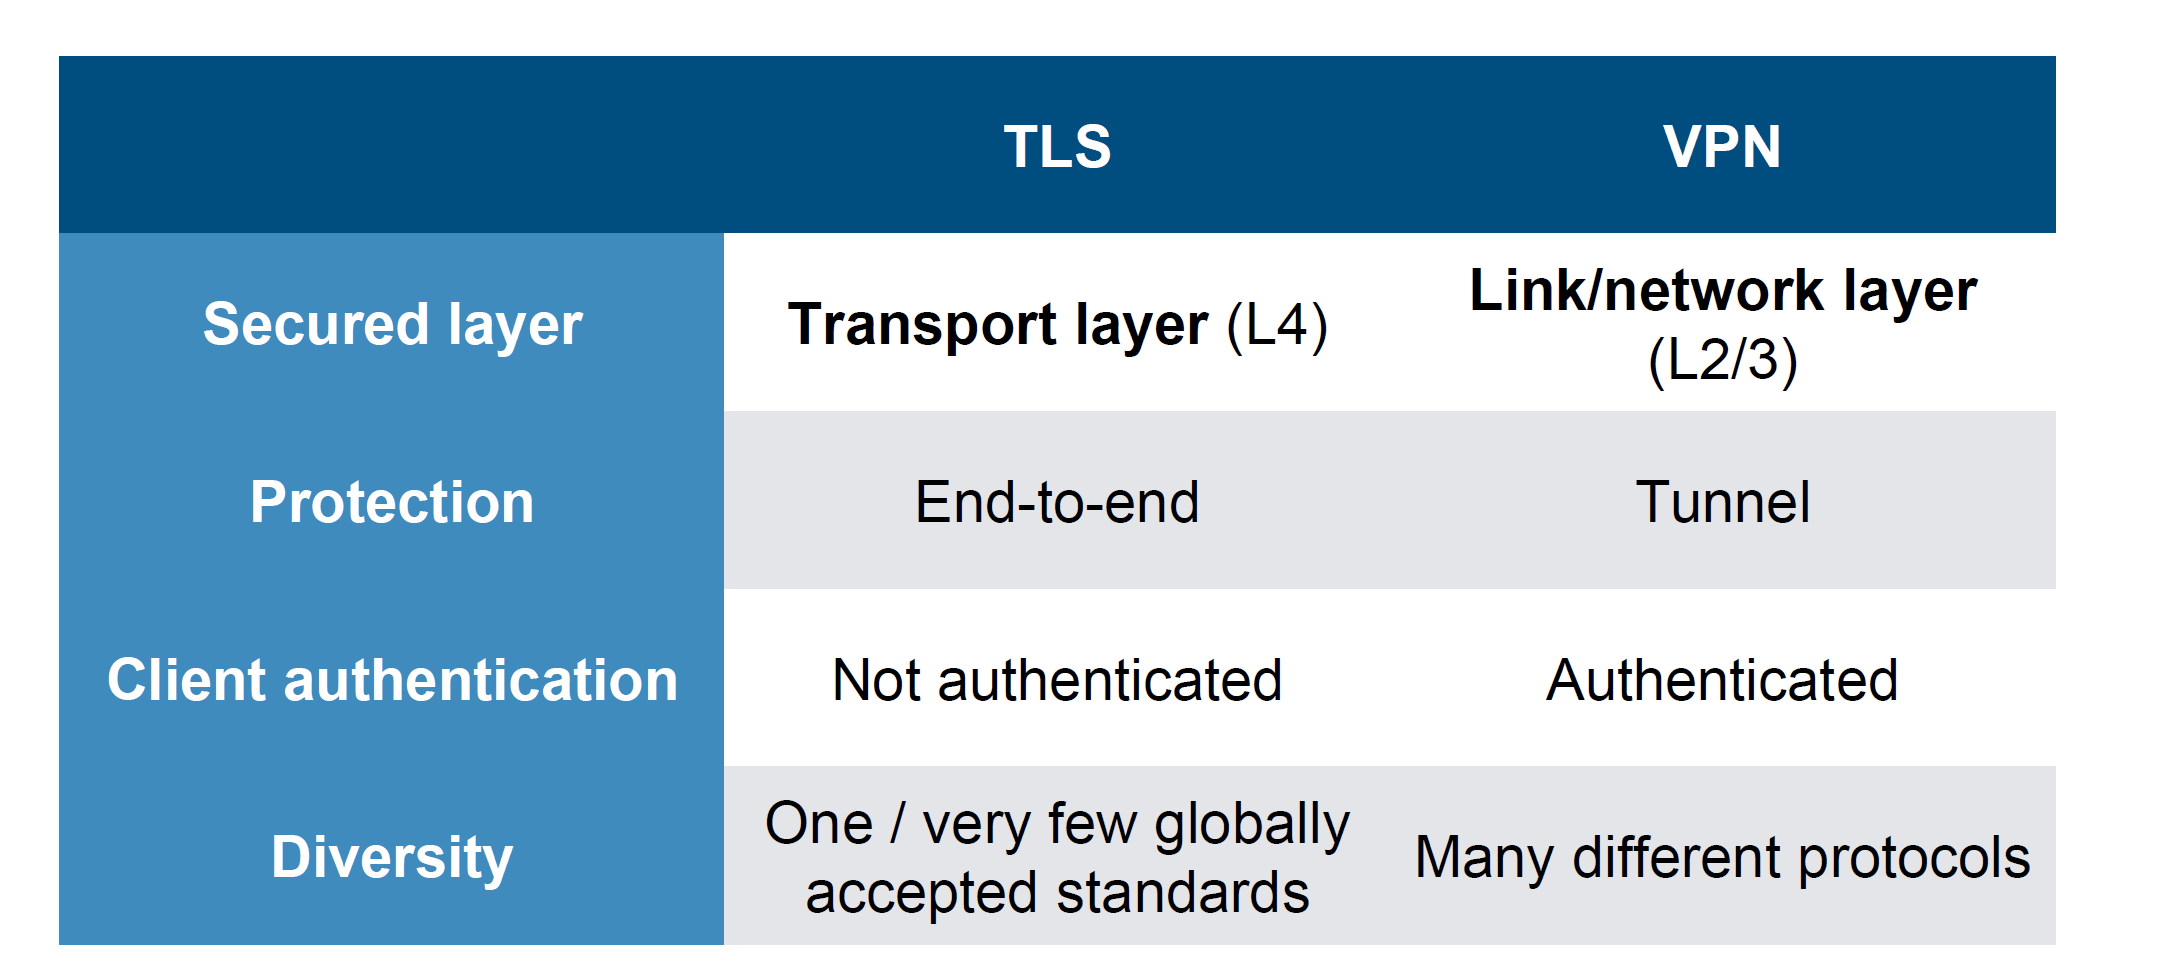
\includegraphics[width=\linewidth]{Figures/VPN_tls.PNG} 
\end{minipage}

\paragraph{Availability/Performance of VPNs:}
\begin{itemize}
    \item VPNs can negatively impact performance (potential detours, limited bandwidth at VPN server, additional crypto)
    \item Generally VPNs do not provide higher availability (no DDoS defence)
    \item VPNs can defend against targeted packet filtering (Routers can recognize VPN packets but not content
\end{itemize}

\paragraph{VPN vs VLAN}
\begin{itemize}
    \item VPN: connects two different networks
    \item VLAN: set up multiple isolated virtual networks on a single physical infrastructure.
\end{itemize}

\textcolor{orange}{Look at schema example of VPN routing on slide 21}

\subsection{IPsec}

\begin{enumerate}
    \item Set up a security association (SA) via IKE
    \item Encapsulate packets and tunnel them between SA endpoints
\end{enumerate}

IPsec is a very large and complicated protocol. The tunnel is setup at layer 3 (network). In IPsec, we also use sequence numbers (like in TLS) \textit{but} they are included in the packets (while TLS doesn't include sequence numbers in the packet). That's because IPsec runs on top of IP and IP is best-effort transport. The ordering of packets can thus be off at the receiver. That's why sequence numbers need to be in the packets. What if we are tunneling UDP traffic?
The numbers are also there to avoid replay attacks. Each party has a sliding window so that it can
detect if a packet is replayed by inspecting the sequence number. IPsec and IKE have many options and modes

\paragraph{Problems with IPsec}
\begin{itemize}
    \item Configuration is difficult and error-prone due to many options.
    \item Some options do not provide any security
\end{itemize}

\subsubsection{Internet key exchange (IKEv2)}

IKE is used to setup a security association (SA). In IKE, we have an anonymous DH exchange. This provides forward security and does not leak identities (as e.g. TLS does) since no authentication data is sent in plaintext. The disadvantage is that anonymous DH is vulnerable to an active MiTM attack.

\begin{minipage}{\linewidth}
    \centering      
    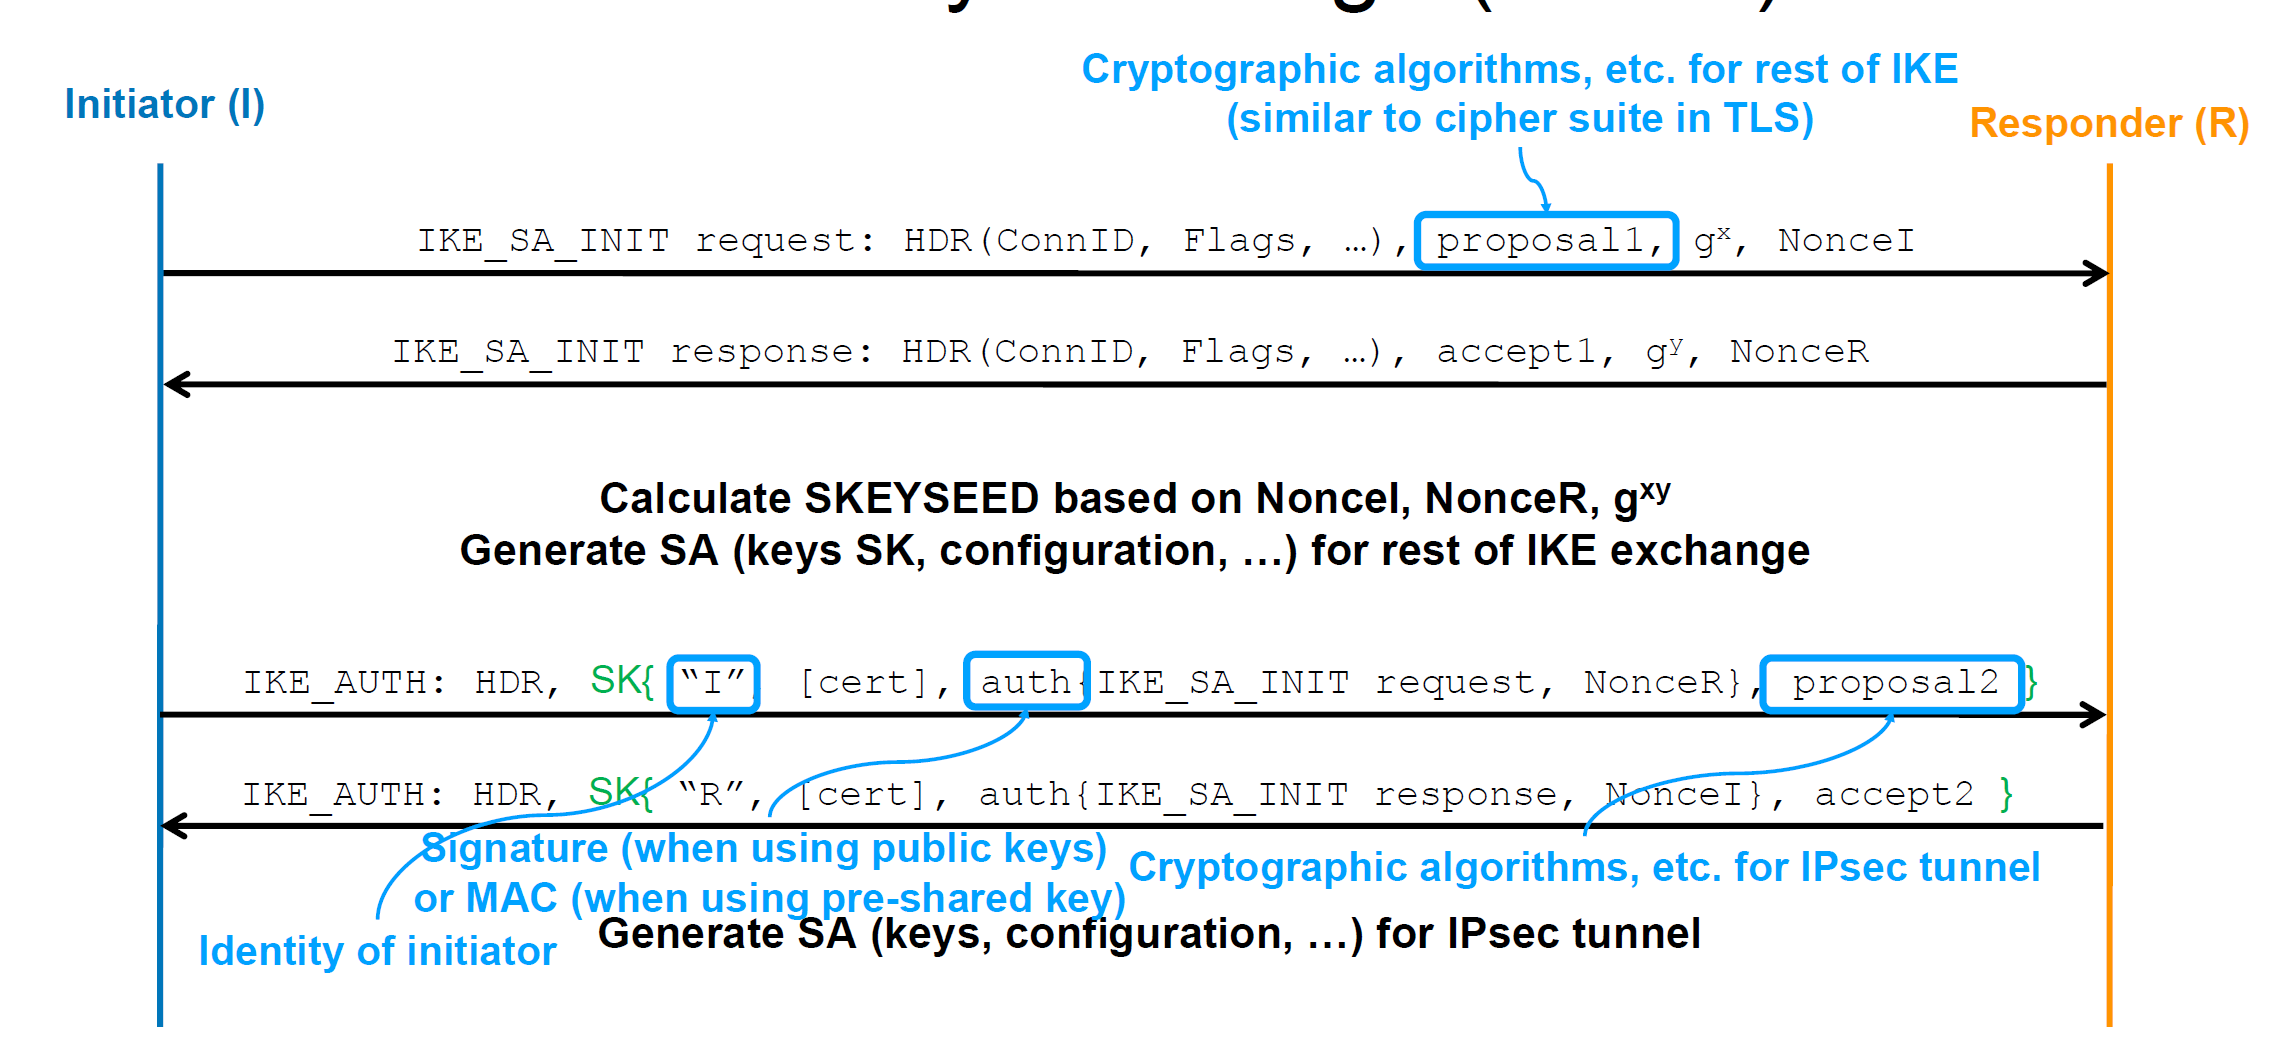
\includegraphics[width=\linewidth]{Figures/VPN_IKE.PNG} 
\end{minipage}

\subsubsection{IPsec session}

After an SA was setup using IKE, we encapsulate packets and tunnel them between SA endpoints. Encapsulation works as follows:

\begin{itemize}
	\item Add ESP trailer: Padding, type encapsulated (original) packet
	\item Encrypt packet and trailer
	\item Add ESP header: SA identification, sequence number
	\item Create Integrity Check Value (ICV): MAC over original packet, ESP	header, ESP trailer
	\item Add new IP header
\end{itemize}

\begin{minipage}{\linewidth}
    \centering      
    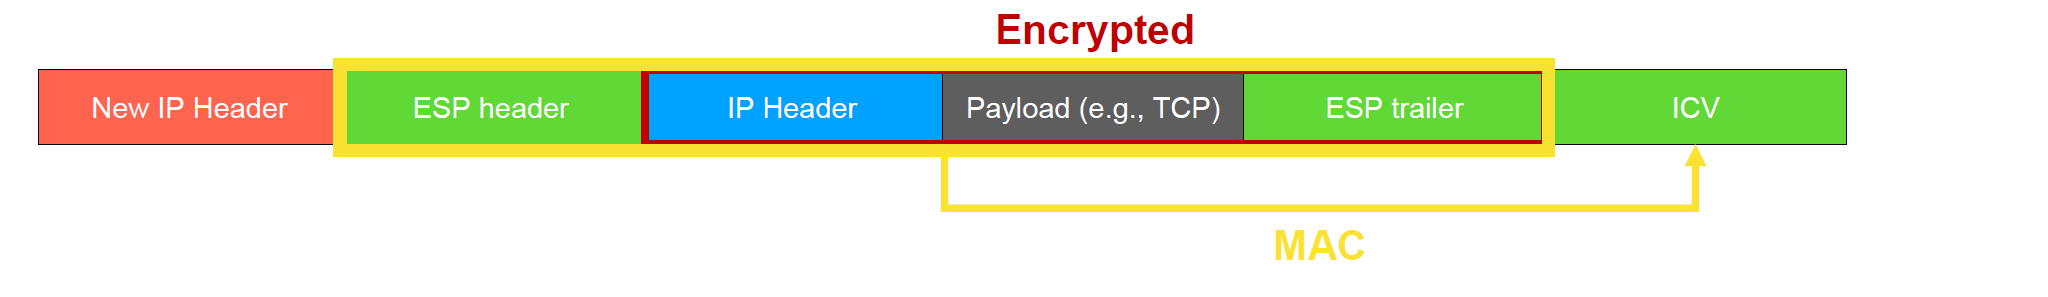
\includegraphics[width=\linewidth]{Figures/VPN_session.PNG} 
\end{minipage}

Similarly, decapsulation:

\begin{itemize}
	\item Strip off outer IP header
	\item Look up keys and configuration using information in ESP header
	\item Check MAC
	\item Strip off authentication tag and ESP header
	\item Decrypt original packet
	\item Remove ESP trailer
	\item Forward original packet
\end{itemize}

\begin{minipage}{\linewidth}
    \centering      
    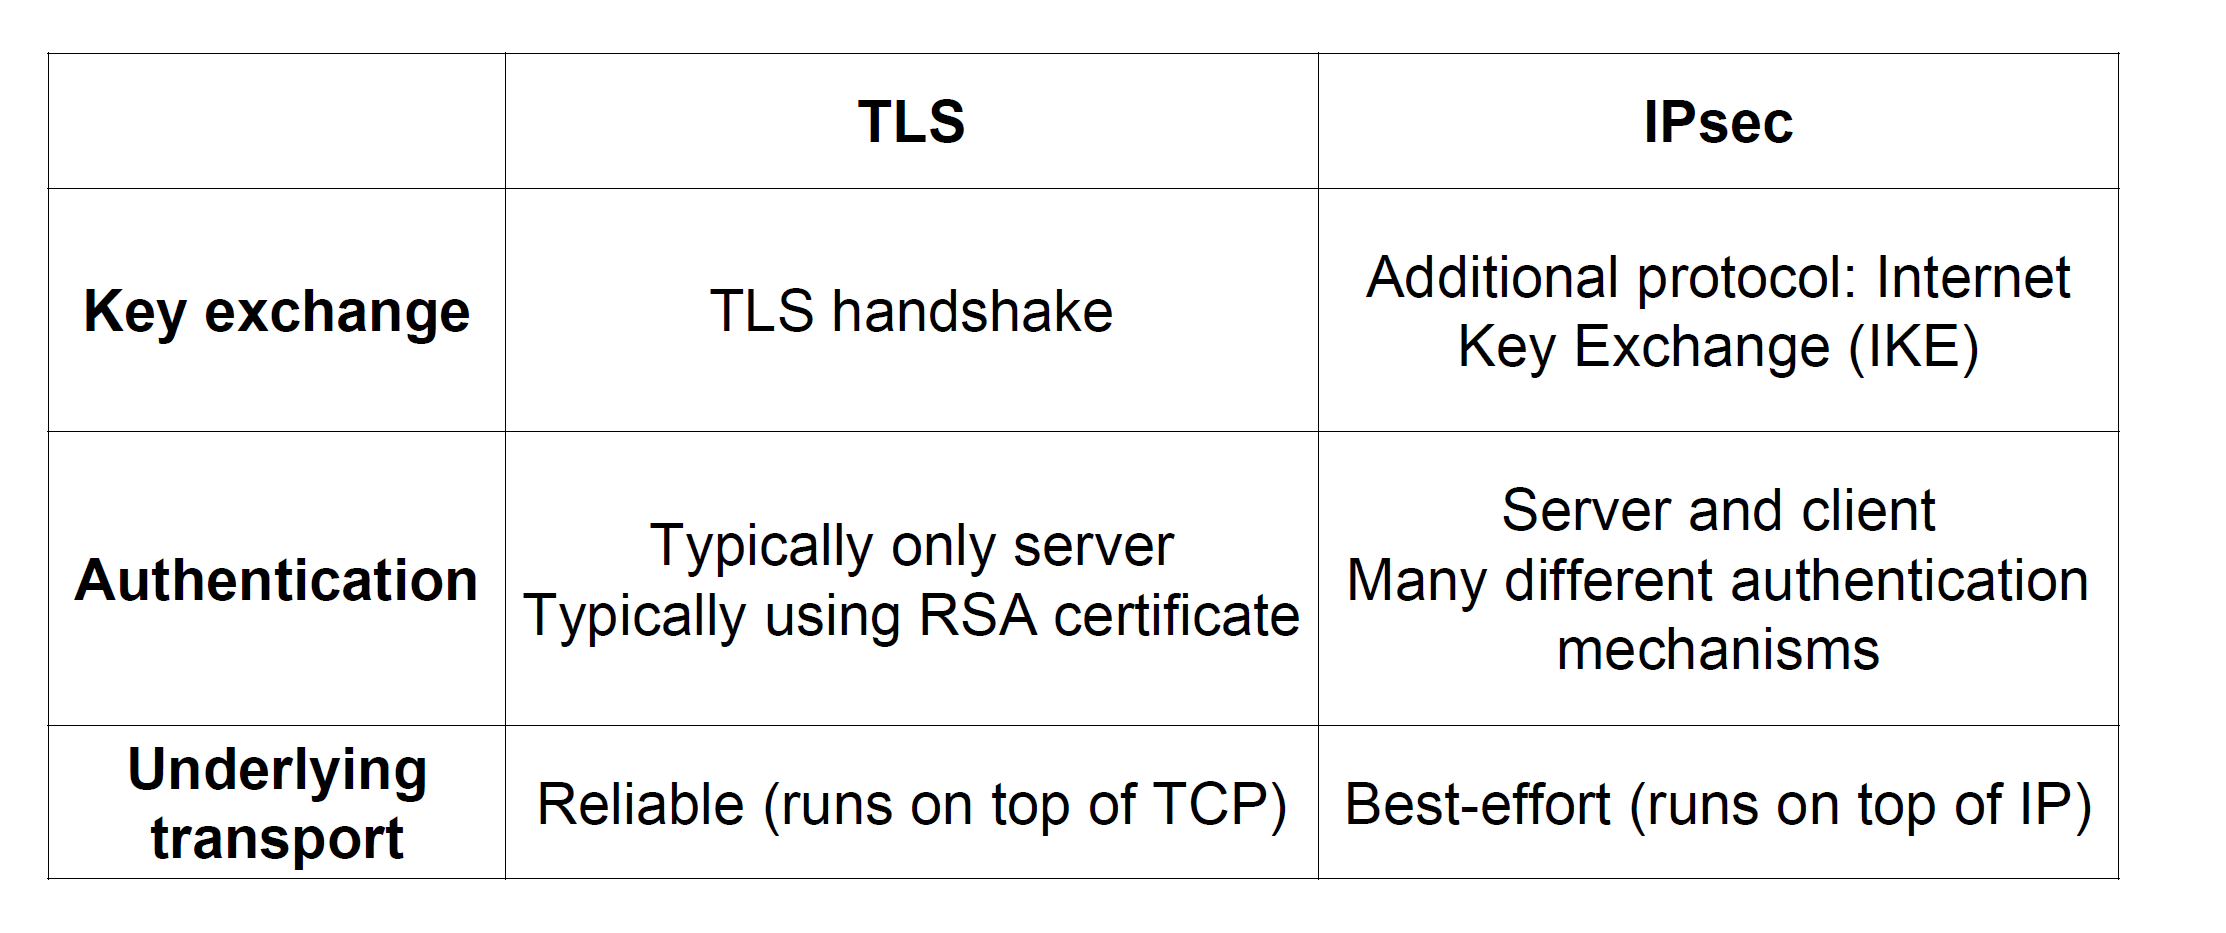
\includegraphics[width=\linewidth]{Figures/VPN_ipsec_tls.PNG} 
\end{minipage}

\subsection{Wireguard}

WireGuard is a modern lightweight VPN that only has roughly 4000 LOC (opposed to OpenVPN with 600'000 LOC!).\\
WireGuard relies on simple configuration and no cryptographic agility. It only uses state-of-the-art primitives: Curve25519 (signatures), ChaCha20 (encryption), Poly1305 (authentication). The small codebase provides minimal attack surface and is formally verifiable. Wireguard is faster than IPsec or OpenVPN. 

\subsubsection{Authentication and keys}

Each peer has a static key pair. Initiator: $S_I^{pub}, S_I^{priv}$, Responder: $S_R^{pub}, S_R^{priv}$. Peers specify in configuration which public keys are authorized. WireGuard uses a 1-RTT handshake during which each peer generates an ephemeral key pair: Initiator: $E_I^{pub}, E_I^{priv}$, Responder: $E_R^{pub}, E_R^{priv}$. Symmetric keys are then derived from four DH combinations: $$\{DH(S_I,S_R), DH(S_I,E_R), DH(E_I,S_R), DH(E_I,E_R)\}$$

\begin{minipage}{\linewidth}
    \centering      
    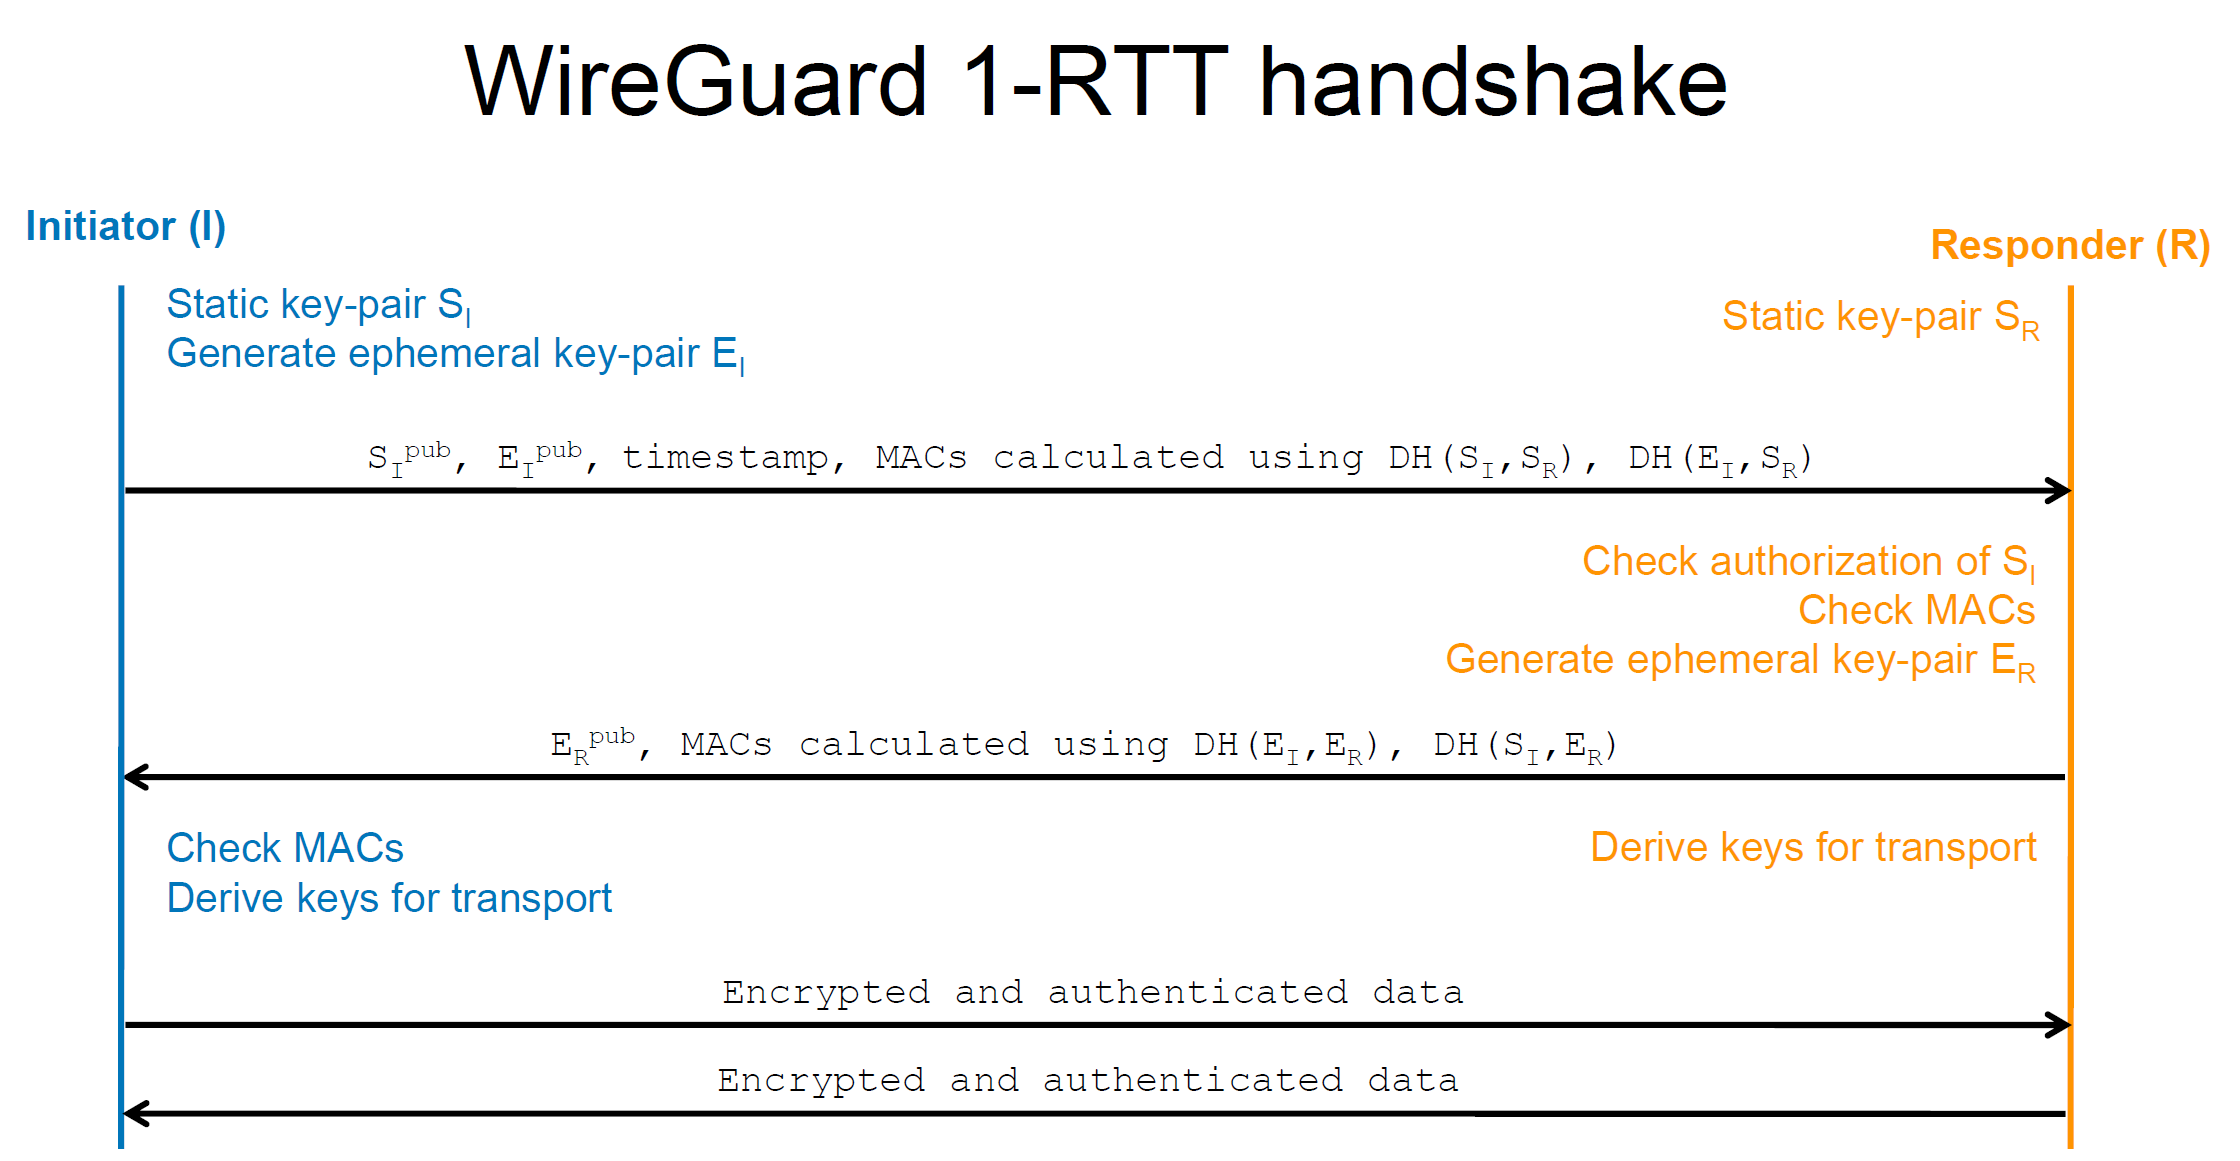
\includegraphics[width=\linewidth]{Figures/VPN_wireguard.PNG} 
\end{minipage}

The WireGuard protocol is connectionless. A series of timers, both based on message counts and time, are used to steer key renegotiation, handshakes and session termination. The strict key rotation timers \texttt{(REKEY\_AFTER\_MESSAGES, REKEY\_AFTER\_TIME)} and the ephemeral
ECDH session key exchange guarantee PFS.

\subsubsection{DoS protection}

Since VPN servers need to do expensive crypto, they are susceptible to (D)DoS attacks. A WireGuard implementation can choose to respond with a cookie instead of processing the handshake: the initiator will then use this cookie as a key for computing HMACs of their message. The cookie mechanism of IKEv2 is very similar to the one just described. However, an important difference between the two is that Wireguard requires an additional MAC on the handshake message — using the public key of the responder as HMAC key. This allows the responder to stay completely silent — not responding even with a cookie — unless the initiator knows its public key. (Remember that “public” key do not need to be publicly accessible, often they are not).


